
\chapter{Bakgrunn}

I dette kapittelet vil de viktigste konseptene, fenomenene og teknologiene bli beskrevet og eksisterende  forskning som er relevant for oppgaven. 

\section{Kommunikasjonsform: Symboler}

De som ikke har mulighet til å bruke skrift som kommunikasjonsform kan bruke tegnsystemer. Det eksisterer tre typer tegnsystemer: håndtegn(manuelle tegn) som innebærer å bruke håndbevegelser, materielle tegn vil si at en bruker fysiske objekter som brikker eller figurer og den siste er; grafiske tegn som innebærer at en bruker symboler. I denne rapporten er vil symboler bli brukt som kommunikasjonsform. Her representerer symboler et ord, frase, uttrykk eller setning. Ifølge ISAAC \cite{Tegnsystemer} er grafiske tegn brukt av mennesker med store bevegelsesvansker som gjør at de har utfordringer med å lage manuelle tegn, og mennesker med forståelsesvansker som følge av lærehemning.

De vanligste grafiske tegnsystemene på markedet er fotografi, pictogram, Picture Communication Symbols(PCS), Widgit, SymbolStix og Bliss \cite{GrafiskTegn}. I prosjektet brukes SymbolStix (se figur \ref{fig:katt}). Grunnen til dette er at Sono Flex bruker dette tegnsystemet.


\begin{figure}[ht!]
\centering
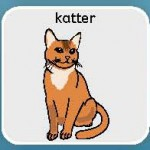
\includegraphics[width=50mm]{katt}
\caption{Et eksempel på et symbol som blir brukt i det grafisk tegnsystemet SymbolStix}
\label{fig:katt}
\end{figure}

\section{Interaksjonsform: Øyestyring}

Menneske-maskin-interaksjon fungerer ved at en person gir maskinen en kommando, og maskinen svarer med en respons. For at et menneske skal kunne gi en maskin ordre, er det nødvendig at maskinen har en inputenhet som tolker beskjedene fra brukeren, slik at at datamaskinen forstår dem.  Som regel er dette tradisjonelle enheter som tastatur og mus. Det eksisterer derimot mangfoldige måter å samhandle med en maskin på. I denne rapporten vil brukerinput bli gitt ved en øyestyringsenhet.  Ved å fange opp brukerens skuepunkt av et videokamera og infrarøde lys, er det mulig for maskinen å beregne hvor på monitoren personen ser. Dette gjør interaksjon mellom dem mulig. En knapp vil for eksempel bli aktivisert ved at brukeren ser på den en hvis periode. 




\section{Forskning}


\subsection{Organisering}


I 1926 kartla Smith\cite{Smith} barns vokabularutvikling fra alderen 1 til 5 år . Resultatene (se tabell \ref{fig:BarnVak}) viste at allerede i en alder av 3 er det vanlig å ha en gjennomsnittlig forståelse for cirka 900 ord. Forskningen er 88 år gammel, men viser omfanget av utfordringen barn har i møte med symbolbasert kommunikasjon. Mens et barn med taleevne kun trenger å finne ordet i hukommelsen, må barn som bruker symboler først finne det og deretter lokalisere det representative symbolet. 

I applikasjonen som skal utvikles vil symbolene bli presentert i en tabell. Antall symboler som får plass i tabellen begrenses av skjermens fysiske størrelse og at de må være store nok til at brukeren har mulighet til å se  og samhandle med dem. En slik tabell med symboler vil herfra bli referert til som en side. For hver setning brukeren vil uttrykke må han navigere seg igjennom flere av disse sidene for å finne symbolene som representerer ordene i setningen. Det er derfor essensielt at organiseringen legger til rette for akkurat dette, og ikke vanskeliggjør barnets evne til å lokalisere, velge og bruke symbolene.

\begin{table}[h]
\begin{tabular}{llllllllll}
\hline
Alder (År, Måneder) & 1 & 1,6 & 1,9 & 2,0 & 2,6 & 3,0 & 3,6  & 4,0  & 5,0  \\ 
Antall ord          & 3 & 22  & 118 & 272 & 446 & 896 & 1222 & 1540 & 2072 \\ 
Økning              & 2 & 19  & 96  & 154 & 174 & 450 & 326  & 330  & 532  \\ \hline
\end{tabular}
\caption{Tabell som viser vokabular vekst hos barn.  Smith \cite{Smith} sitert av Dale \cite{Dale} }
\label{fig:BarnVak}
\end{table}



Drager og Light \cite{aac} viser til at det inntil nylig var gjort lite forskning på layouts og organisering for barn eller om faktorene som spiller inn når det gjelder lokalisering og bruk av målobjektene. Målobjektet er symbolet som brukeren ønsker å uttrykke. Wilkinson og Jageroo \cite{Wilkinson2006} har undersøkt hvilke påvirkning farge har som en faktor når det kommer til organisering og hvordan elementer skal fordeles. De kom frem til at fargehint spiller en viktig rolle innen visuell prosessering  og hukommelse. Ved å legge til en farge ved elementene i tabellen over symboler, påvirket det nøyaktigheten og effektiviteten til barn i 4-5 års alderene i å finne målobjekt. Eksempelvis kan man gi symboler som representerer verb en grønn farge, adjektiv en blå, pronomen gul o.s.v. Fenomenet kalles Fitzergald Key og gjør at barn mer presist og raskere lokalisere målobjektet. Scally \cite{Scally} argumenterer for at farge ikke nødvendigvis er den eneste variabelen som må vurderes. Andre skjerm variabler som kan påvirke læring og bruk er: bakgrunn, kanter/grenser, form, tekstur, størrelse, posisjon, bevegelse og animasjon. Videre undersøkelser må til for å avgrense effektene av disse funksjonene for å kunne optimere designet til ask-systemer.


\subsection{Navigasjon}
\label{subsec:navigasjon}

Hvis en tar med alle typene frukt så vil det ikke være plass til alle symbolene på en side, dette gjør at de må deles opp over flere sider.Konsekvensen er at brukeren må ha mulighet til å navigere mellom disse sidene for å finne ønsket symbol. Siden antallet symboler det er plass til på hver side begrenses av skjermstørrelsen og brukerens syn, er spørsmålet hvor mange symboler bør plasseres på hver side med tanke på effektivitet. Drager og light med kollegaer undersøkte nettopp dette. Resultatene indikerte at barn i alderen 2-5 hadde større vanskeligheter for å lokalisere korrekt side fra en meny med 4 symboler enn en så lokalisere målobjektet når på korrekt side ut av et valg på 12 til 30 symboler, til tross for at sannsynligheten for å finne korrekt side er 25 prosent er mye større enn å finne korrekt symbol 0.03 - 0.08 når en først er på rett side.

For barn kan det å navigere være ekstra vanskelig. Dette kommer av flere grunner: (a) de må ha en konseptuell modell av de gjemte sidene i systemet i minnet. Med andre ord forstå hvordan de mest effektivt kan komme seg fra forsiden til ønsket symbol. (b) De må forstå forholdet mellom representasjon brukt på menysiden og de gjemte sidene i vokabularet. Er det symbolet som har bilde av et kjøkken eller av en butikk som leder til symbolet eple? I denne rapporten vil disse utfordringene bli undersøkt.


